\documentclass[11pt]{article}

\usepackage{hyperref}
\usepackage{url}
\usepackage{graphicx}
\usepackage{amssymb}
\usepackage{geometry}[margins=1in]
\graphicspath{ {./images/} }


\title{\textbf{Weather Translation in Images Using Variational Autoencoders}}
\author{Stefan Stefanache}

\begin{document}
    \maketitle

    \section{Hypothesis}
    In this paper, the weather translation task is proposed, which 
    refers to transferring weather conditions of the image from one category 
    to another. It is important for photographic style transfer. This has been 
    attempted before through WeatherGAN \cite{DBLP:journals/corr/abs-2103-05422}, where weather 
    conditions are determined by various weather-cues, obtained through 
    attention and segmentation modules, which are then passed to a translation module 
    that generates a new image. Our hypothesis is that convolutional variational autoencoders 
    can be trained to give better (more realistic) results in this task, by 
    using a specialized dataset containing paired (from the same POV) images with different
    weather conditions. \textbf{Disclaimer:} Currently, the paper describes the dataset and
    its construction, specifically for the sunny/cloudy cases, along with a draft proposal
    for the VAE model architecture. The code is available at 
    \href{https://github.com/thesstefan/vae_weather_translation}
    {github.com/thesstefan/vae\_weather\_translation}.
    and the dataset is available 
    \href{https://drive.google.com/file/d/1q7OjUZgz2ZzPzfsHPzbNluJye450oid9/view?usp=share_link}
    {here}.
    \section{Related Work}

    In this section, we introduce some state-of-the art approaches of weather recognition
    and image-to-image translation, as well as a brief discussion on datasets created 
    for various tasks related to weather.

    \subsection{Weather Recognition}
    Elhoseiny et al. \cite{7351424} tackles the two-class weather classification 
    task by the AlexNet \cite{10.1145/3065386}, which has got superior performance 
    than handcrafted features. Moreover, to combine the advantages of deep feature 
    and handcrafted feature, these two kinds of features are integrated 
    in \cite{7784804}. The multi-task model proposed by 
    Zhao et al. \cite{ZHAO2019272} identifies weather cues in images through segmentation
    and then uses them to classify images, achieving state-of-the-art performance.

    \subsection{Weather Datasets}

    One popular dataset for weather recognition is called \textbf{MWI} \cite{7351637, ZHANG2016365}
    (Multiclass Weather Image). It contains 20K images obtained from many web albums and 
    films, such as Flicker, Picasa, Poco, Fengniao. The images are collected 
    by several helpers, and they choose images with their own common sense. The main 
    purpose of this dataset is to provide an extensive testbed for the evaluation of 
    existing appearance models, and provide insight needed to develop new appearance models.

    To facilitate weather property estimation from images, a large-scale image dataset 
    associated with rich weather information called \textbf{Image2Weather} \cite{7545010} 
    was developed. Based on the taken time and geographical information of an image, 
    weather properties obtained from a weather forecast website are linked with the images. 
    Through data filtering like indoor/outdoor classification and sky region detection, 
    the dataset consisting of more than 180,000 photos is built to promote related research.
    
    \subsection{Image-To-Image Translation}

    Studies have explored various models with GANs for image-to-image translation.
    For example, Pix2pix, used a conditional, generative adversarial network 
    \cite{DBLP:journals/corr/MirzaO14} for image translation, when a source and target image 
    pair was given. Similar methods have been adopted for several tasks, such as synthesizing 
    a photograph from a sketch \cite{DBLP:journals/corr/SangkloyLFYH16}. Weather translation
    was also approached using GANs, through WeatherNet \cite{DBLP:journals/corr/abs-1910-09910}.

    When paired training data were not available for some tasks, other studies have 
    suggested several approaches to transform from an unpaired image. This has been approached
    from both the perspective of coupled GANs (UNIT \cite{DBLP:journals/corr/LiuBK17}),
    and by using cross-domain variational encoders and decoders \cite{DBLP:10.3390/app9224780}.

    \section{Our Approach}

    In this paper, we propose an image-to-image translation framework for the
    weather translation task, using CVAEs (convolutional variational autoencoders)
    powered by a specialized dataset (called \textbf{weather2weather}), created for
    this purpose.

    \subsection{The weather2weather Dataset}

    The \textbf{weather2weather} dataset is constructed from scratch by ourselves. 
    It consists of \textbf{TBD} (currently around 5000) images scraped 
    from \href{windy.com}{windy.com}, a provider of webcam streams. Images are separated 
    by the webcam streams they belong from, so one can create pairs of images from 
    the same location, which can then be used for paired image-to-image translation 
    tasks related to weather. Weather-cues for each image are extracted in a segmentation 
    mask using the multi-task weather recognition model proposed in \cite{ZHAO2019272},  
    which are then used to assign a weather label to the image. The process of 
    constructing the dataset is illustrated in \ref{fig:dataset}. Stream images and 
    their inferred properties are also cleaned and verified by the authors, who 
    check for misclassifications or unsuitable images using tools like the 
    one shown in \ref{fig:dataset_tool}. 

    Currently, the model only classifies images into sunny or cloudy. The model could also be
    extended for multiclass classification for other cases like foggy, snowy or rainy weather.
    The process of enhancing the \textbf{weather2weather} dataset could be automated further
    by handling some edge cases, like detecting noisy images or webcams that are moving. 

    \begin{figure}[!htb]
        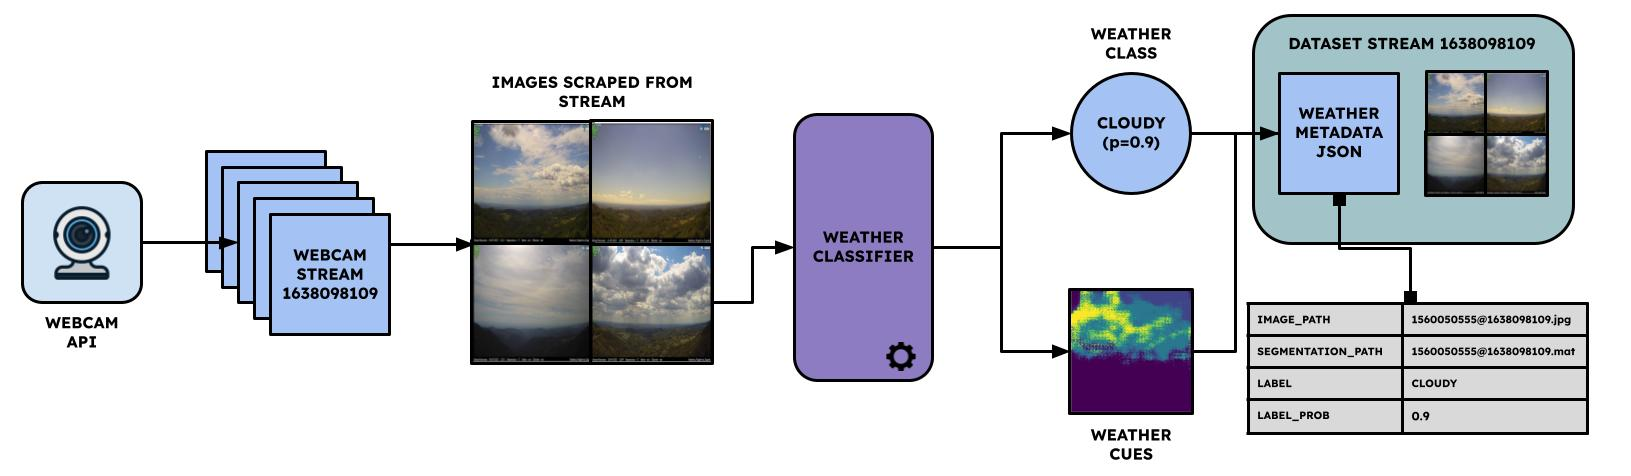
\includegraphics[width=\linewidth]{images/dataset_assembly.jpg}
        \caption{Creating the \textbf{weather2weather} dataset}
        \label{fig:dataset}
    \end{figure}

    \begin{figure}[!htb]
        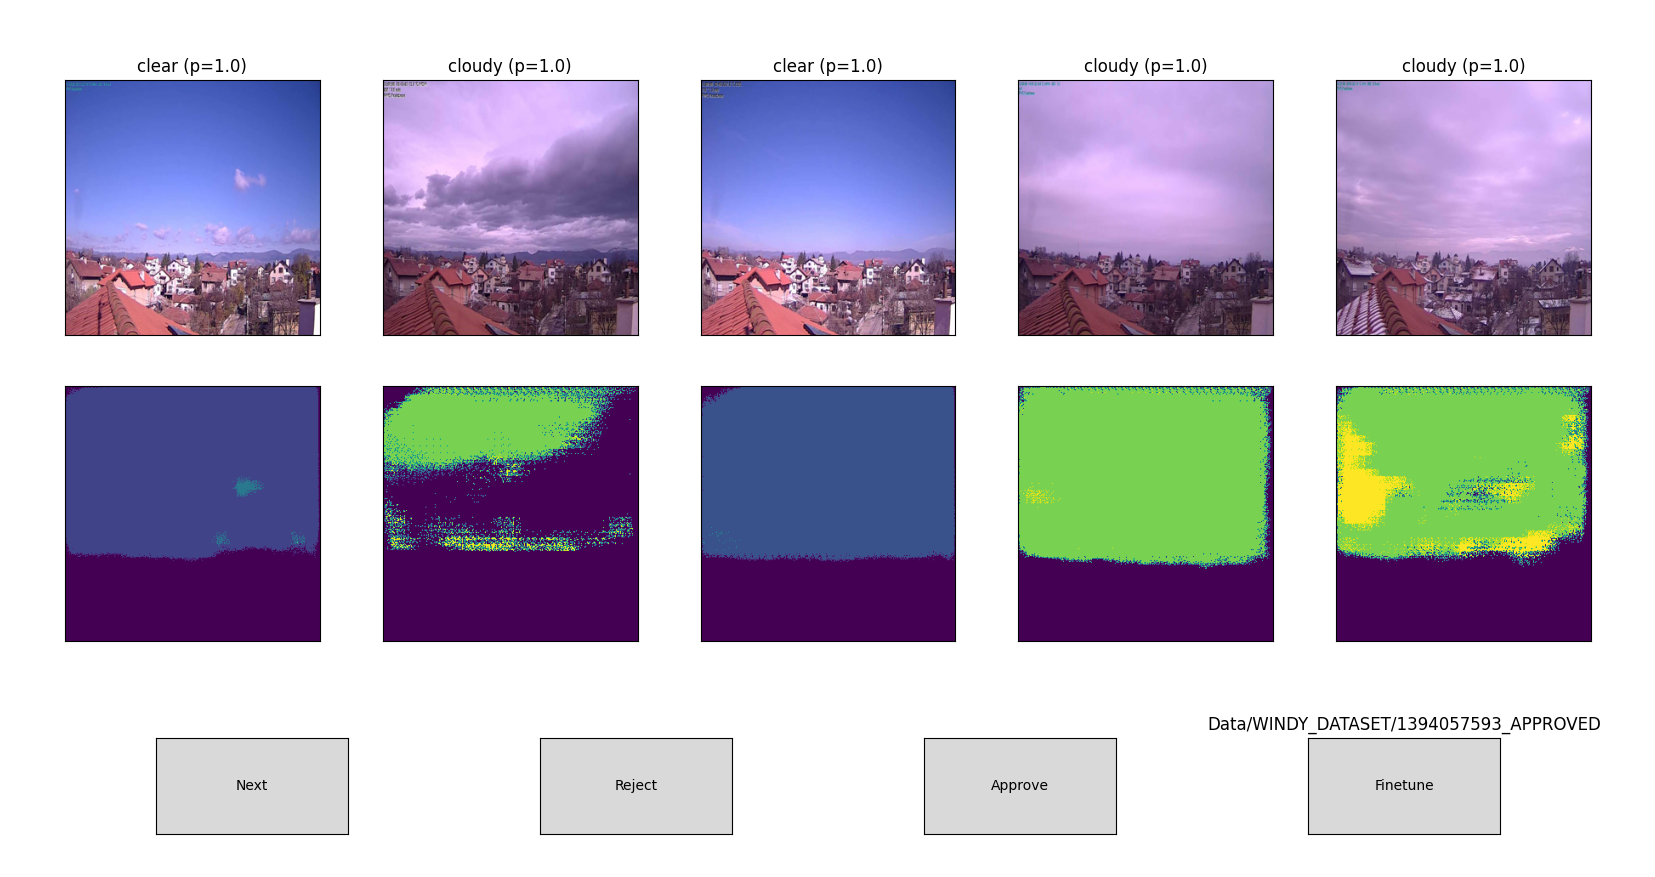
\includegraphics[width=\linewidth]{images/dataset_tool.png}
        \caption{Validating streams in the \textbf{weather2weather} dataset}
        \label{fig:dataset_tool}
    \end{figure}

    \subsection{Weather-To-Weather Translation Model}

    \textbf{Disclaimer:} Exact model architecture and training details \textbf{TBD}.
    
    Convolutional variational auto-encoders are used to learn about the distribution
    of images and weather cues (segmentation masks) for each weather category (currently
    cloudy or sunny). The bottlenecks of both decoders are then merged through a composition
    (\textbf{TBD}) operation. The model samples a data sample from the resulting distribution,
    which then is taken through a decoder that produces the translated image. Note that
    each decoder is also trained on a corresponding weather category. Generally, the 
    decoders and encoders used are chosen based on the input image weather category and
    the target weather category.

    The train data is obtained by taking each pair of images with different weather categories
    from every stream in the \textbf{weather2weather} dataset, resulting in over 15000 such pairs.
    Train images and segmentations masks are pulled through the model. To train the auto-encoders
    and decoders for each domain, we follow the basic equation of the convolutional
    auto-encoder \cite{https://doi.org/10.48550/arxiv.1312.6114}. The representation
    of the $k$-th latent feature map extraction for input $I$ is denoted as
    \begin{equation}
        h^k = \sigma(I * W^k + b^k)
    \end{equation}
    where $\sigma$ is an activation function, $W_k$ is a weight, $b^k$ is a bias,
    and $*$ represents the 2D convolution operation. The reconstruction of the latent
    representation is obtained using 
    \begin{equation}
        y = \sigma\bigg(\int_{k \in H} h^k * \widehat{W} + c\bigg)
    \end{equation}
    where $c$ is a bias for input channel. The model is trained to minimize the ELBO loss
    \cite{https://doi.org/10.48550/arxiv.1312.6114}, which is defined as
    \begin{equation}
        \min \mathbb{E}_q[\log q(z | x) - \log p(z)] - \mathbb{E}_q \log p(x | z)
    \end{equation}
    where the first term is the Kullback-Leibler divergence and the second term is 
    the construction loss.

    The first step of translation is taking an image and inferring its weather cues
    and weather label using the model proposed by \cite{ZHAO2019272}. Based on the
    classification label, the corresponding encoders are used to compress the image
    and its segmentation mask to produce the merged latent space. A sample then is taken
    from the merged sample space to produce the translated image using the corresponding
    encoder. The process is illustrated in \ref{fig:model}.

    \begin{figure}[!htb]
        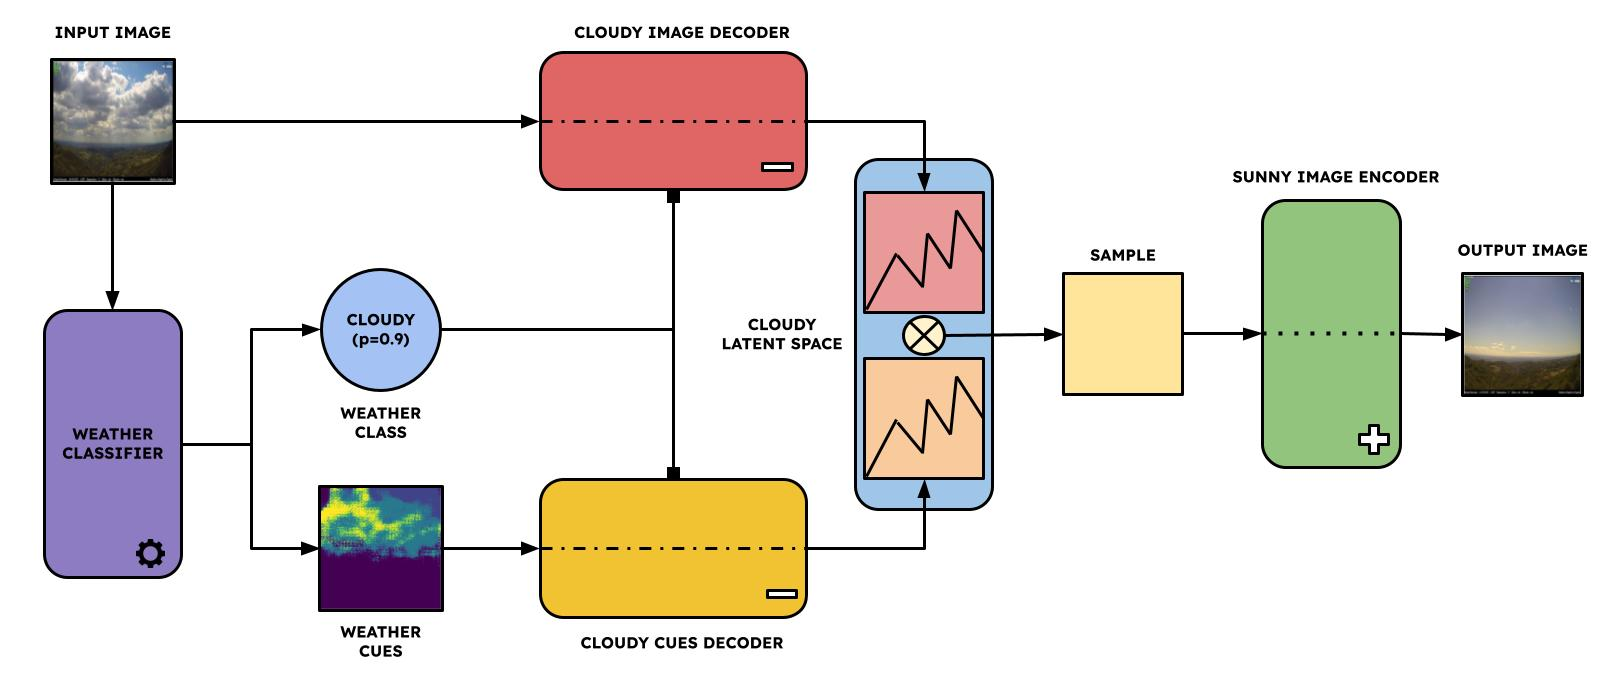
\includegraphics[width=\linewidth]{images/model_architecture.jpg}
        \caption{The weather translation process}
        \label{fig:model}
    \end{figure}



    \section{Methodology}

    To achieve this result, we follow the steps below:

    \begin{enumerate}
        \item Create dataset containing pictures from the same angle and different weather conditions, 
            labelled with weather categories. 
            \begin{enumerate}
                \item Scrape images from \href{windy.com}{windy.com} webcams from 
                    year-round slide show. These contain images with all kinds of 
                    weather (foggy, snowy, sunny, cloudy), taken from the same POV (see Fig. \ref{fig:windy}).
                \item Drop images of streams having defects like a lot of noise or high variations in 
                    scenery (rarely, webcams can be moved to another location).
                \item Develop a ResNet-based \cite{DBLP:journals/corr/HeZRS15} network similar to WeatherNet 
                    \cite{DBLP:journals/corr/abs-1910-09910} to label each image with the 
                    corresponding weather category.
            \end{enumerate}
            Assuming that stream images are from the same physical locations,
            it's likely that the only differences beteween images is given by the changes in scenery 
            caused by time of the year and weather conditions. This allows autoencoders to "learn"
            what this difference is and reproduce it.
        \item Create and train autoencoders for each possible translation (e.g. sunny $\to$ cloudy). 
            For the training, we follow the next steps for each ordered pair of images
            from the same stream in the dataset:
            \begin{enumerate}
                \item Based on the labels of the images, choose the coresponding autoencoder.
                    For example, if the images have the sunny and cloudy labels,
                    use the autoencoder that transforms sunny images to cloudy ones.
                \item Train the chosen encoder to transform from one image to the other e.g.
                    give one image as input of the decoder, and the other as the target output
                    of the decoder.
            \end{enumerate}
            This way, we should end up with a set of encoders that can be merged into model
            that can reliably perform weather translations.
    \end{enumerate}

    \section{Experiments}
    To check how performant our model is, we'll separate some of our dataset into a test portion, 
    and we'll be be evaluating the model's accuracy on it using 2 metrics traditionally 
    \cite{https://doi.org/10.48550/arxiv.2206.10935} used for 
    quantifying the quality of image generative models:
    \begin{enumerate}
        \item Frechet Inception Distance (FID) \cite{https://doi.org/10.48550/arxiv.1706.08500}: 
            The score summarizes how similar the two groups are in 
            terms of statistics on computer vision features of the raw images calculated using 
            the Inception v3 model used for image classification. Lower scores indicate the two groups 
            of images are more similar, or have more similar statistics, with a perfect score 
            being 0.0 indicating that the two groups of images are identical.
        \item Kernel Inception Distance (KID): Calculates the square of the maximum average difference 
            between the two sets of images (input  and output), which represents the distribution 
            distance between the two sets of data. In addition, KID has an unbiased estimator, 
            which makes KID close to human perception.
    \end{enumerate}

    Moreso, this metrics can be used to compare the performance of our model with others 
    like Pix2Pix \cite{DBLP:journals/corr/IsolaZZE16}, NVIDIA's UNIT \cite{DBLP:journals/corr/LiuBK17}  
    or WeatherGAN \cite{DBLP:journals/corr/abs-2103-05422}.

    \begin{figure}[!htb]
        \minipage{0.499\textwidth}
            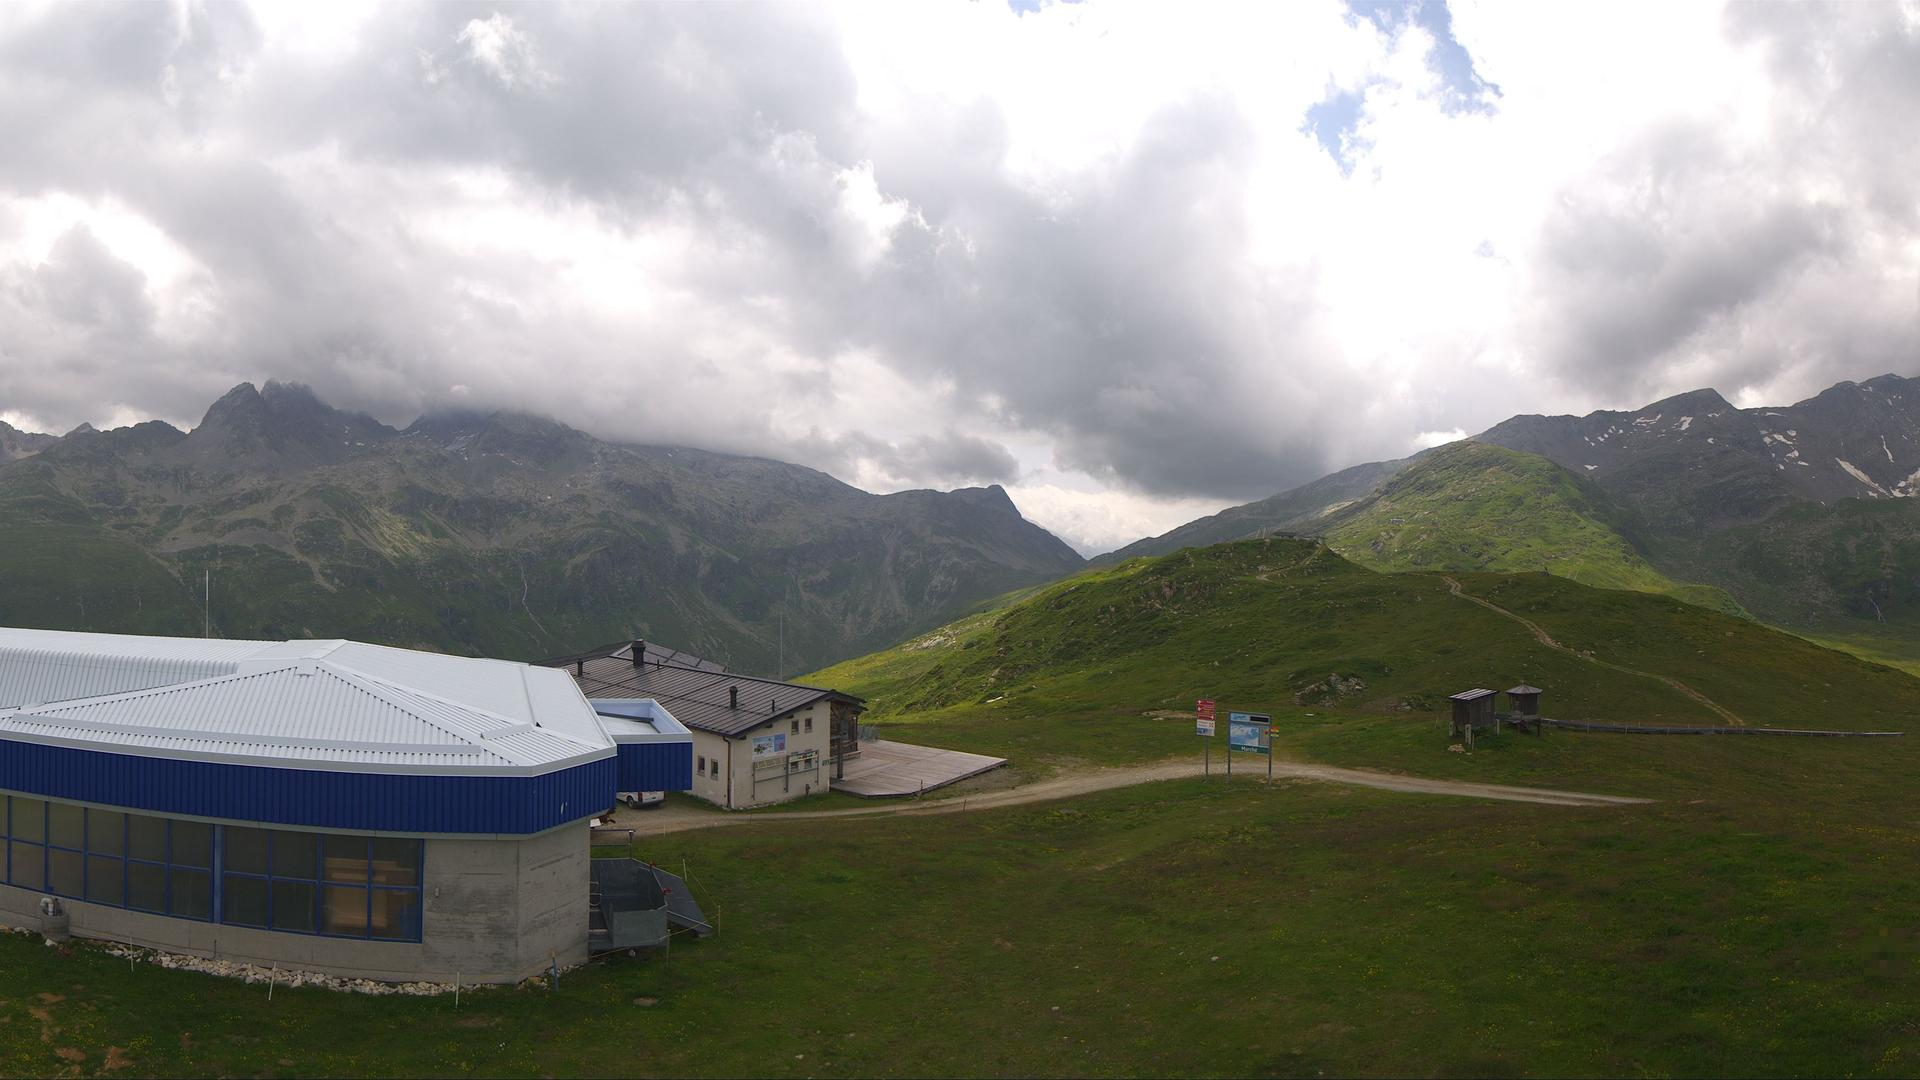
\includegraphics[width=\linewidth]{images/1_cloudy.jpg}
        \endminipage\hfill
        \minipage{0.499\textwidth}
            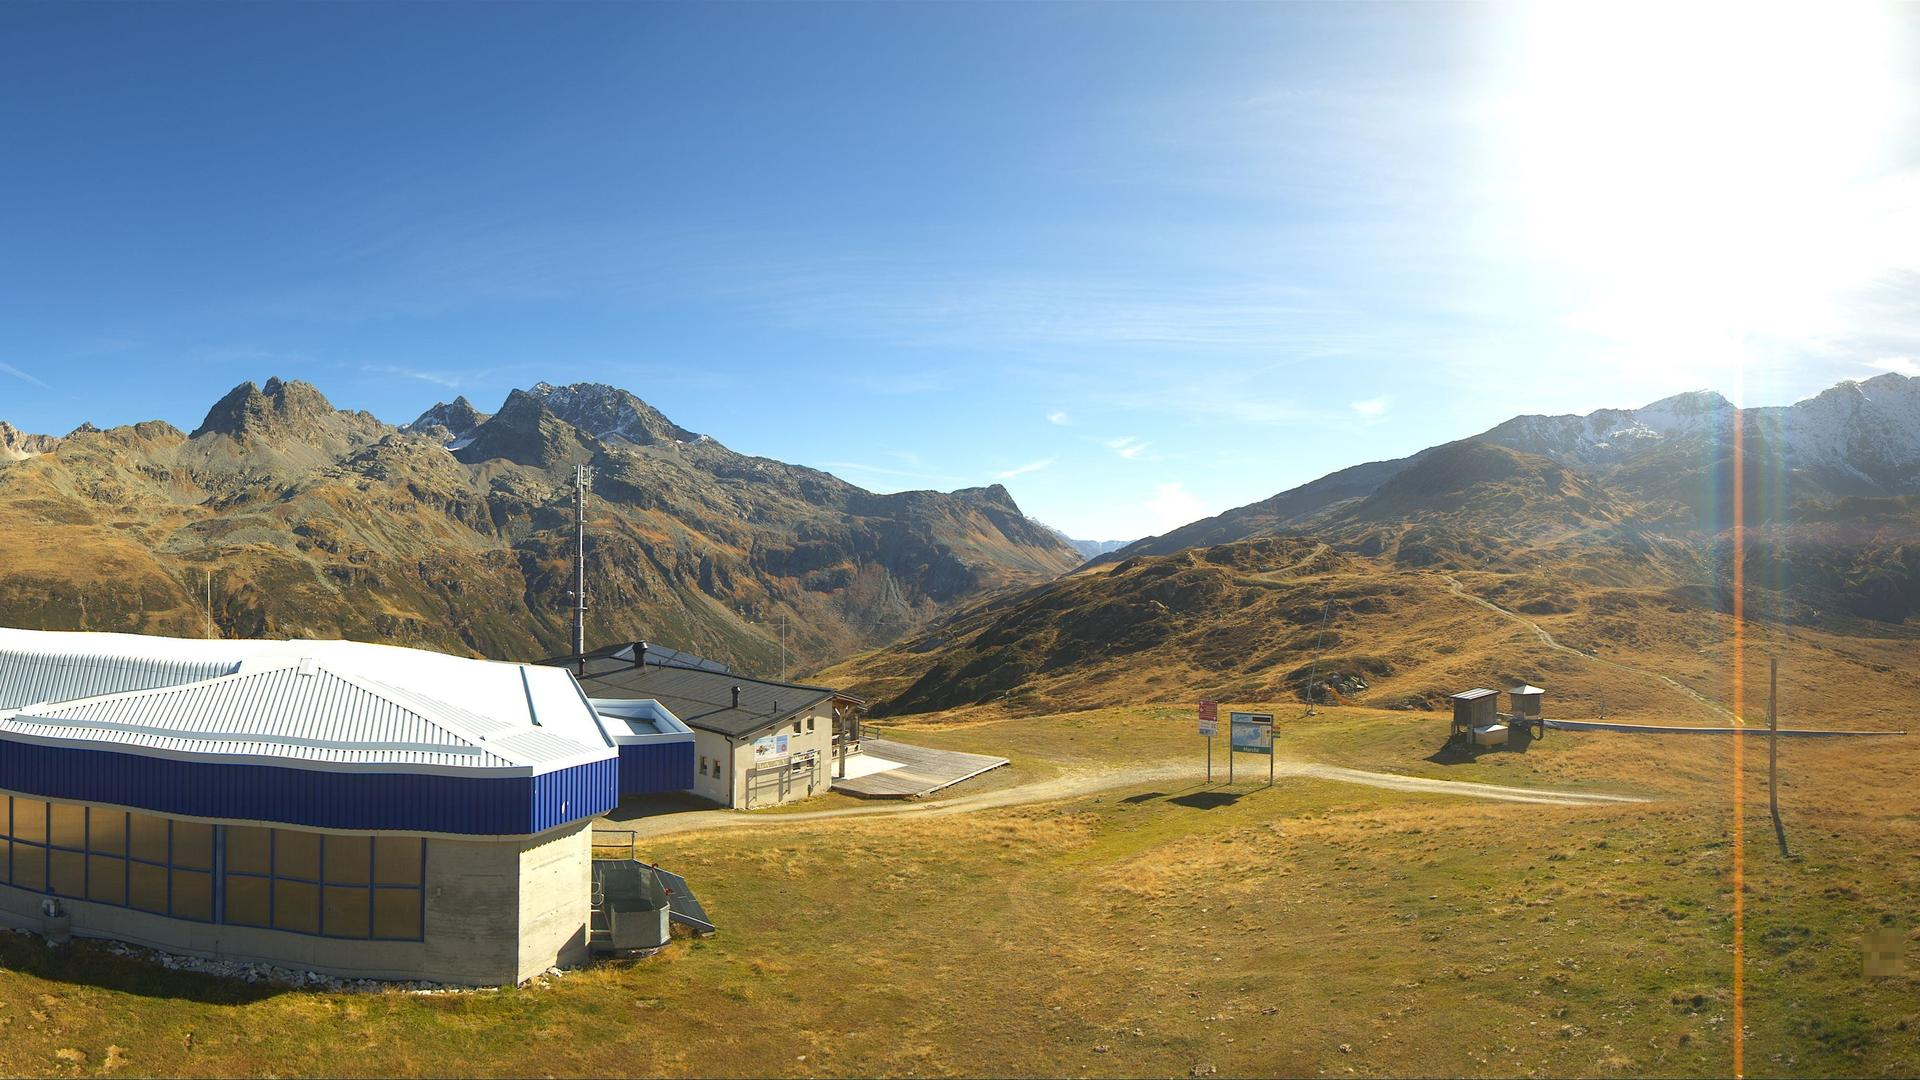
\includegraphics[width=\linewidth]{images/2_sunny.jpg}
        \endminipage\hfill
        \minipage{0.499\textwidth}
            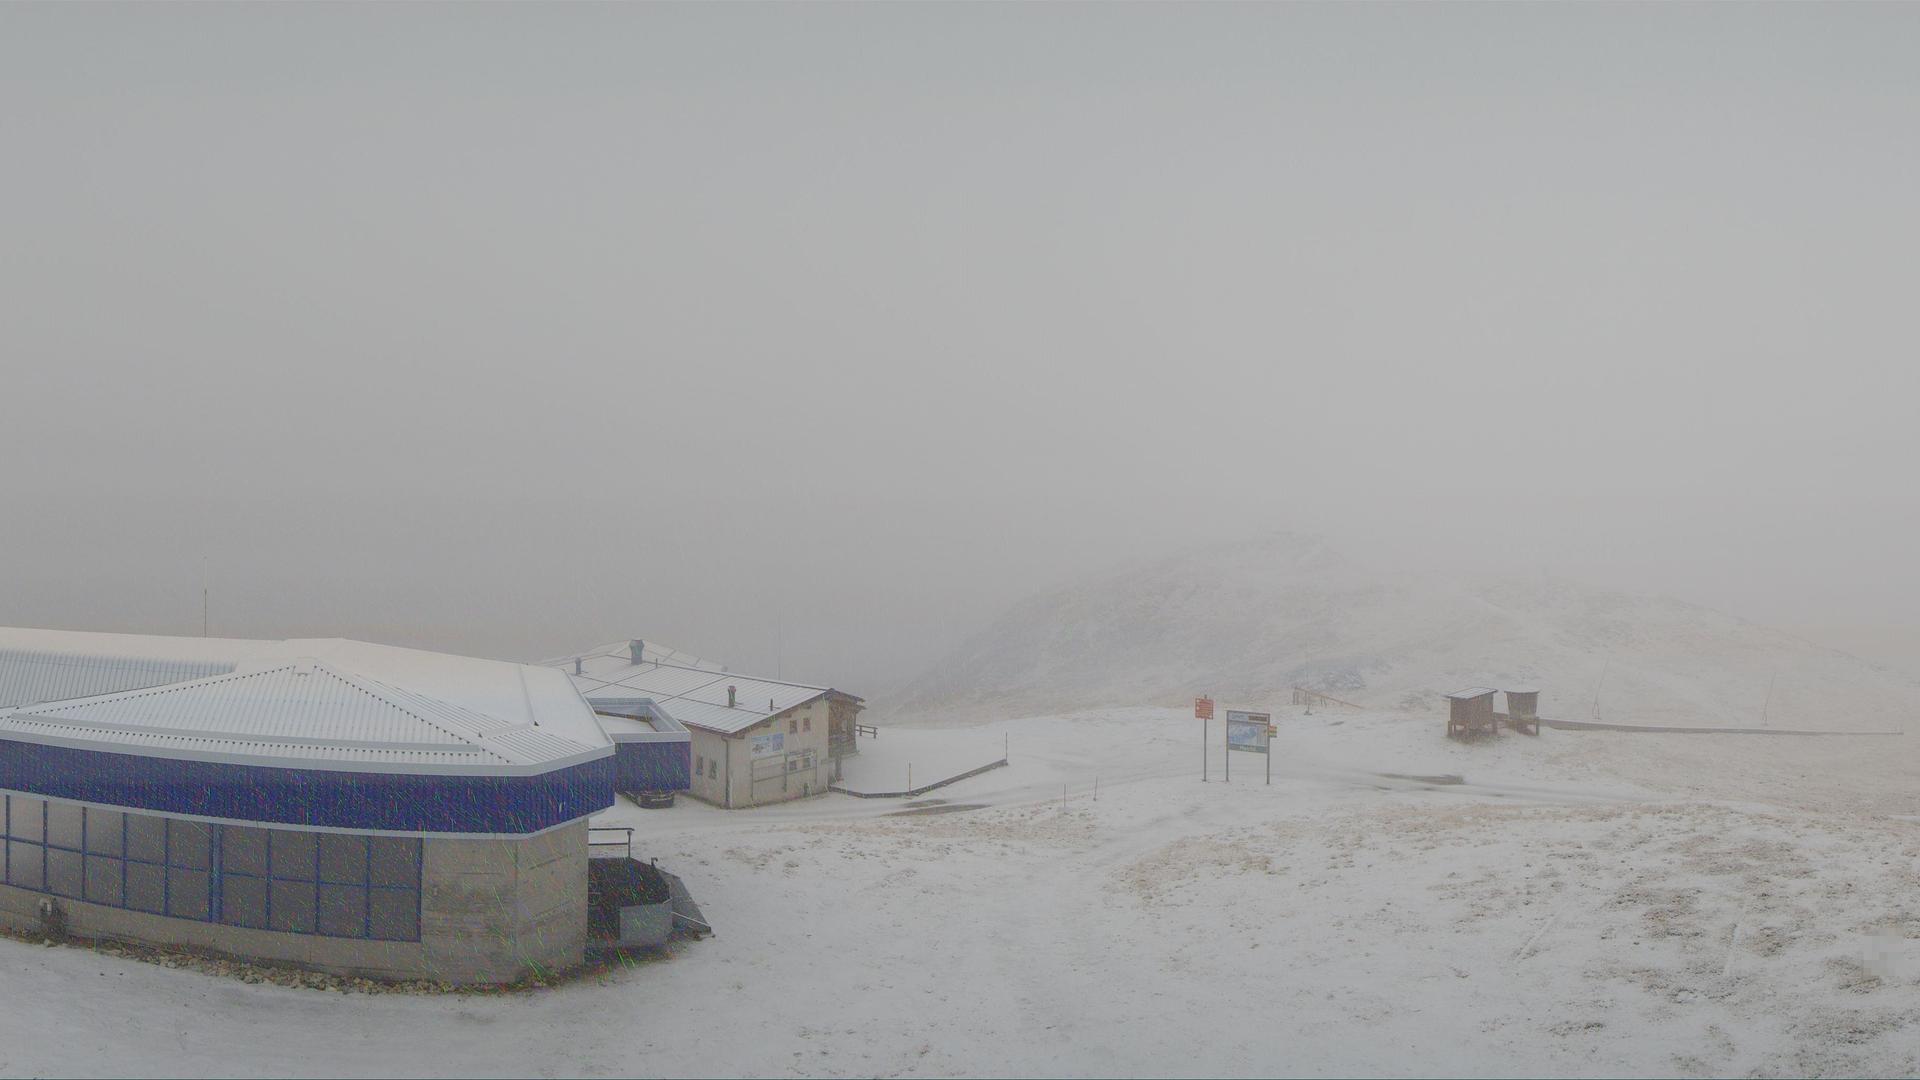
\includegraphics[width=\linewidth]{images/3_snowy_foggy.jpg}
        \endminipage\hfill
        \minipage{0.499\textwidth}
            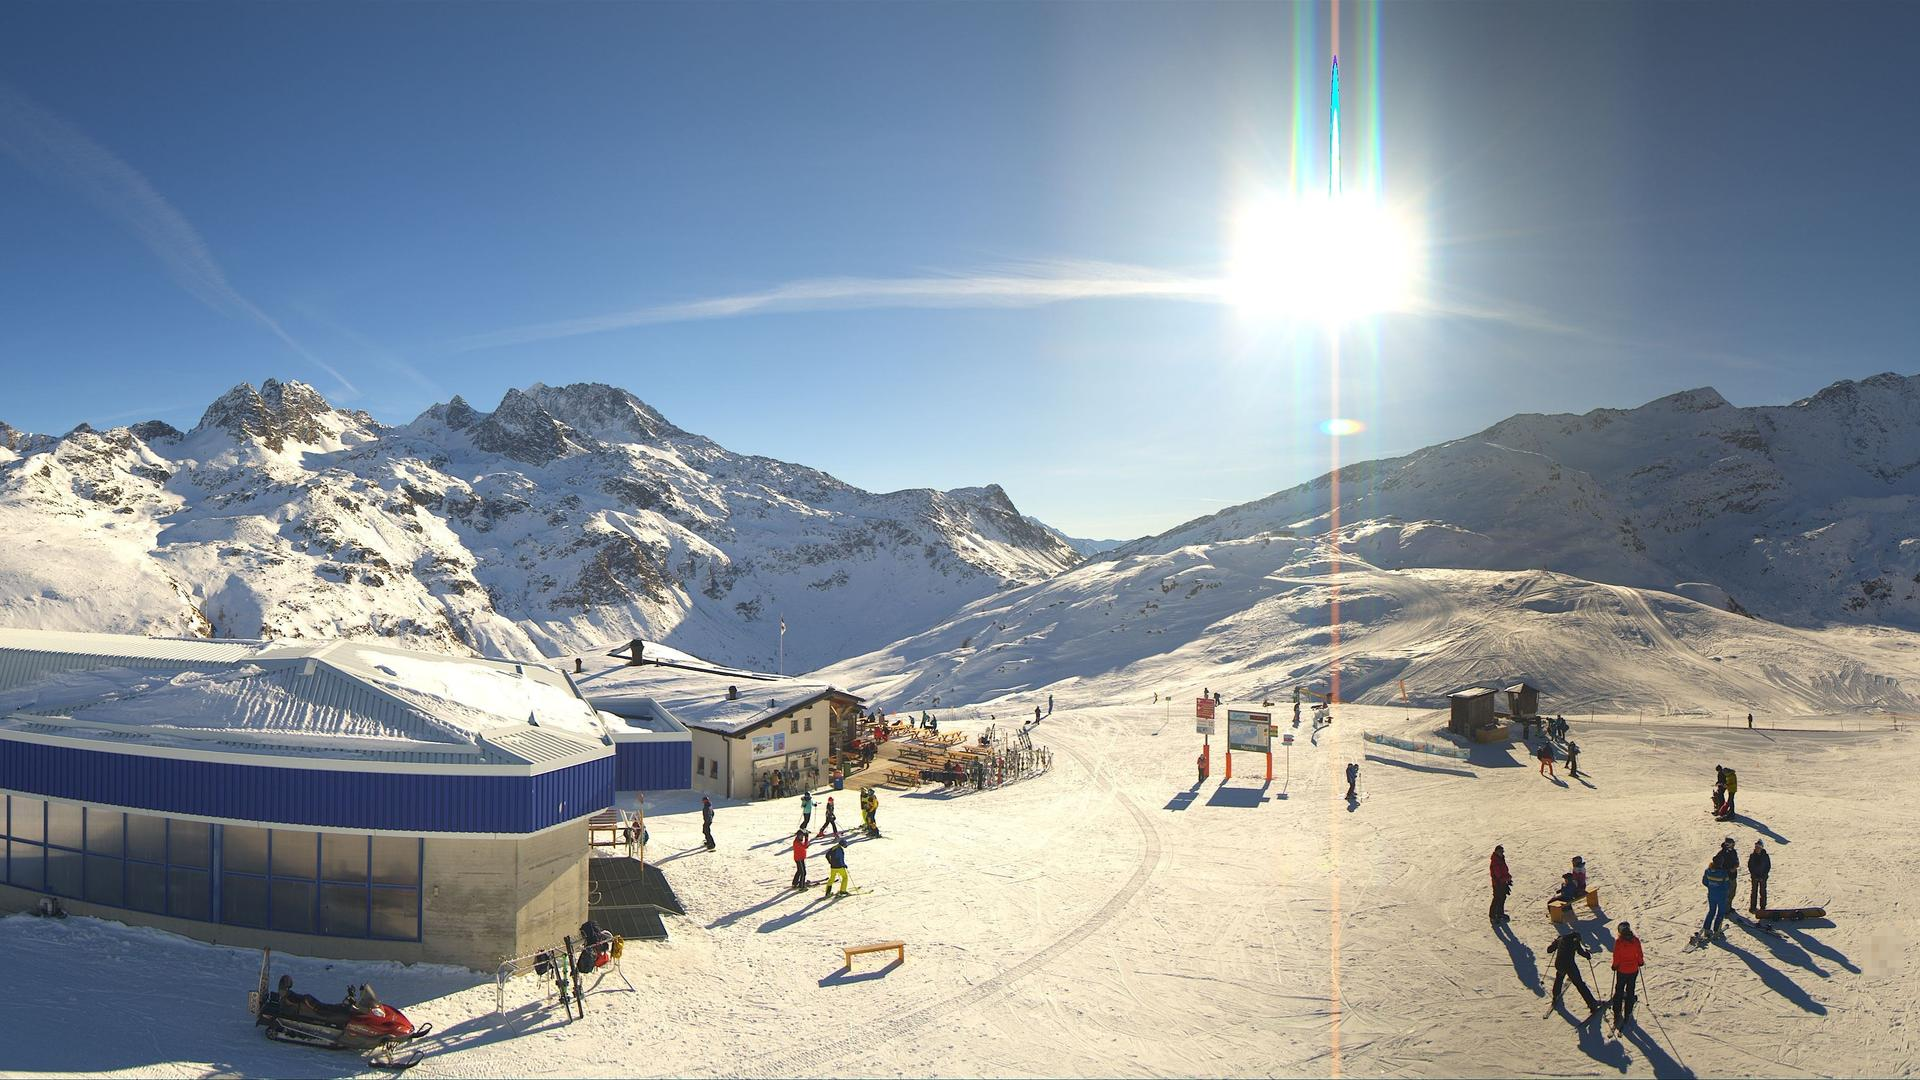
\includegraphics[width=\linewidth]{images/4_snowy_sunny.jpg}
        \endminipage\hfill
        \caption{Images from the Splugen Tanatzhöhe Ski Area webcam from \href{windy.com}{windy.com}}
        \label{fig:windy}
    \end{figure}

    \section{Reference Motivation}
    \begin{enumerate}
        \item \textbf{ML Concepts \& Neural Networks.}
            Learn more about ML theory and algorithms, along with how Neural Networks are used.
            Bishop's PRML \cite{bishop:2006:PRML} gives an overview of general ML topics and intoduces 
            Neural Networks in Chapter 5. Goodfellow's \cite{Goodfellow-et-al-2016} book gives an introductive 
            overview of Deep Learning. Specific Neural Networks architectures like ResNet 
            \cite{DBLP:journals/corr/HeZRS15} or GANs \cite{https://doi.org/10.48550/arxiv.1406.2661}
            are useful for understanding previous weather recognition and image translation approaches.
        \item \textbf{Weather Recogniton using ResNet.}
            Study previous approaches 
            \cite{DBLP:journals/corr/abs-1910-09910, DBLP:journals/corr/abs-1904-10709, 
            DBLP:journals/corr/abs-2103-05422} of recognizing weather conditions in images using different
            ResNet architectures. Either try to use/implement one of the papers or come up with a slight variation.

        \item \textbf{Variational Encoders.}
            Learn about Variational Encoders and the theory behind them: original paper 
            \cite{DBLP:journals/corr/abs-1906-02691}, introductive overview 
            \cite{https://doi.org/10.48550/arxiv.1312.6114}.
        \item \textbf{Image Translation.}
            Study how image translation is done, from generic frameworks like Pix2Pix 
            \cite{DBLP:journals/corr/IsolaZZE16} or NVIDIA's UNIT \cite{DBLP:journals/corr/LiuBK17},
            to the weather specific case - WeatherGAN \cite{DBLP:journals/corr/abs-2103-05422}.
    \end{enumerate}

    \section{Selected References}
    \subsection{Deep Residual Learning for Image Recognition \cite{DBLP:journals/corr/HeZRS15}}
    \begin{itemize}
        \item \textbf{Summary:} Offers an overview of residual learning and the ResNet architecture. Useful
            for recognizing weather conditions in images and constructing the dataset. 
        \item \textbf{138531 Citations} and \textbf{49 References} (IEEE style)
        \item \textbf{Chapters:}
            \begin{enumerate}
                \item Introduction
                \item Related Work
                \item Deep Residual Learning
                \item Experiments
                \item References
            \end{enumerate}
    \end{itemize}

    \subsection{WeatherNet: Recognising weather and visual conditions from street-level \cite{DBLP:journals/corr/abs-1910-09910}}
    \begin{itemize}
        \item \textbf{Summary:} A pipeline of four deep Convolutional Neural Network (CNN) models, so-called 
            the WeatherNet, is trained, relying on residual learning using ResNet50 architecture, to extract 
            various weather and visual conditions such as Dawn/dusk, day and night for time detection, and 
            glare for lighting conditions, and clear, rainy, snowy, and foggy for weather conditions.
        \item \textbf{33 Citations} and \textbf{39 References} (IEEE style)
        \item \textbf{Chapters:}
            \begin{enumerate}
                \item Introduction
                \item Related Work
                \item WeatherNet Frameworks 
                \item Results 
                \item Discussion 
                \item Remarks and Future Work
                \item Acknowledgement
                \item References
            \end{enumerate}
    \end{itemize}

    \subsection{An Introduction to Variational Autoencoders \cite{DBLP:journals/corr/abs-1906-02691}}
    \begin{itemize}
        \item \textbf{Summary:} Variational autoencoders provide a principled framework
            for learning deep latent-variable models and corresponding
            inference models. In the paper, an introduction
            to variational autoencoders and some important extensions is provided
        \item \textbf{1077 Citations} and \textbf{213 References} (IEEE style)
        \item \textbf{Chapters:}
            \begin{enumerate}
                \item Introduction
                \item Variational Autoencoders 
                \item Beyond Gaussian Posteriors 
                \item Deeper Generative Models 
                \item Conclusion 
                \item Acknowledgement
                \item References
            \end{enumerate}
    \end{itemize}

    \subsection{Unsupervised Image-to-Image Translation Networks \cite{DBLP:journals/corr/LiuBK17}}
    \begin{itemize}
        \item \textbf{Summary:} Unsupervised image-to-image translation aims at learning a joint distribution of
            images in different domains by using images from the marginal distributions in
            individual domains. Since there exists an infinite set of joint distributions that
            can arrive the given marginal distributions, one could infer nothing about the joint
            distribution from the marginal distributions without additional assumptions. To
            address the problem, a shared-latent space assumption is made and an
            unsupervised image-to-image translation framework based on Coupled GANs is proposed.
        \item \textbf{2359 Citations} and \textbf{29 References} (IEEE style)
        \item \textbf{Chapters:}
            \begin{enumerate}
                \item Introduction
                \item Assumptions 
                \item Framework
                \item Experiments
                \item Related Work 
                \item Conclusion and Future Work 
                \item Network Architecture
                \item Domain Adaptation
            \end{enumerate}
    \end{itemize}

    \subsection{Weather GAN: Multi-Domain Weather Translation Using Generative Adversarial Networks \cite{DBLP:journals/corr/abs-2103-05422}}
    \begin{itemize}
        \item \textbf{Summary:} A new task is proposed, namely, weather translation, which refers to 
            transferring weather conditions of the image from one category to another. It is important
            for photographic style transfer. Although lots of approaches have been proposed in traditional 
            image translation tasks, few of them can handle the multi-category weather translation task, since 
            weather conditions have rich categories and highly complex semantic structures. To address 
            this problem, a multi-domain weather translation approach based on generative 
            adversarial networks (GAN) is developed, denoted as Weather GAN, which can achieve the transferring of 
            weather conditions among sunny, cloudy, foggy, rainy and snowy. Specifically, the weather 
            conditions in the image are determined by various weather-cues, such as cloud, blue sky, 
            wet ground, etc.
        \item \textbf{9 Citations} and \textbf{50 References} (IEEE style)
        \item \textbf{Chapters:}
            \begin{enumerate}
                \item Introduction
                \item Related Work
                \item Our Approachj
                \item Experiments
                \item Conclusion 
                \item References 
            \end{enumerate}
    \end{itemize}

    \section{Paper Classification}
    \begin{enumerate}
        \item \textbf{ACM}
            \begin{enumerate}
                \item I.2.10:  Vision and Scene Understanding
                \item I.4.8:  Scene Analysis
            \end{enumerate}
        \item \textbf{AMS}
            \begin{enumerate}
                \item 68T07.  Artificial neural networks and deep learning 
                \item 68T45.  Machine vision and scene understanding
            \end{enumerate}
    \end{enumerate}

    \section{Paper Outline}
    \begin{enumerate}
        \item Abstract
        \item Introduction
            \begin{enumerate}
                \item Motivation and Overview
                \item Contributions
            \end{enumerate}
        \item Background
            \begin{enumerate}
                \item Related Works
            \end{enumerate}
        \item Our Approach
            \begin{enumerate}
                \item Dataset Creation
                \item Model Architecture
                \item Training
            \end{enumerate}
        \item Experiments
            \begin{enumerate}
                \item Results
                \item Comparison with Other Models
                \item Failure Cases
            \end{enumerate}
        \item Conclusion
        \item References
    \end{enumerate}


    \bibliography{references}
    \bibliographystyle{plain}

\end{document}
